\chapter{Experiment Setup}
%%%%%%%%%%%%%%%%%%%%%%%%%%%%%%%%%%%%%%%%%%%%%%%%%%%%
% Overview
%%%%%%%%%%%%%%%%%%%%%%%%%%%%%%%%%%%%%%%%%%%%%%%%%%%%
\section{Overview}
 
%\subsection{Accelerator}
\begin{figure}[!ht]
 \begin{center}
  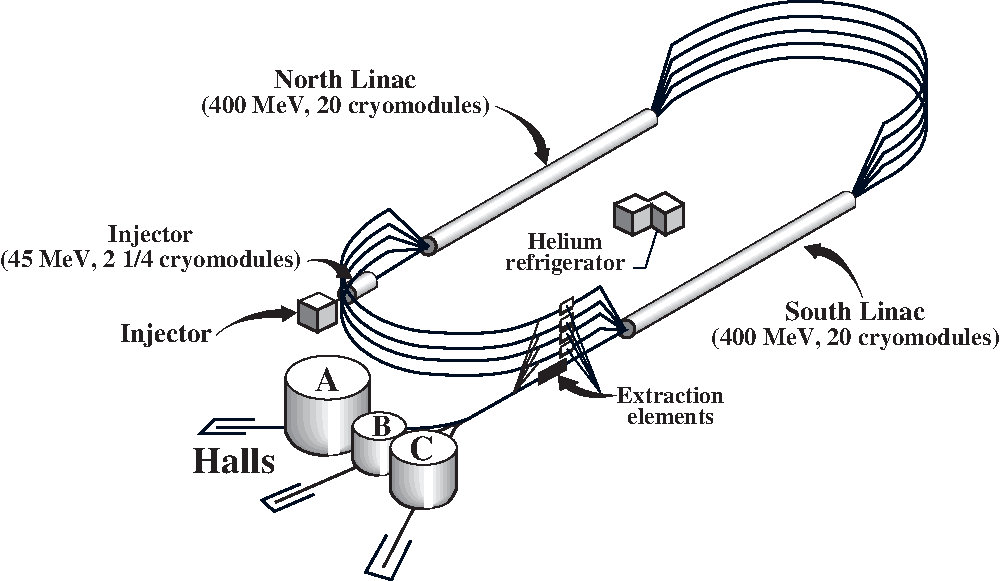
\includegraphics[width=0.55\textwidth]{./figures/halla_jlab/CEBAF}
  \caption[The Accelerator (CEBAF) at JLab]{The Accelerator (CEBAF) at JLab. Figure is from Ref.~\cite{halla_nim}.}
  \label{cebaf}
 \end{center}
\end{figure}
Thomas Jefferson Lab (JLab) is the world's leading medium energy electron scattering laboratory, consisting of a continuous electron beam accelerator facility (CEBAF), three experimental halls (A, B and C), a free electron laser facility and several applied research centers (Fig.~\ref{cebaf}). An upgrade project has been proceeding to increase the beam energy from 6 GeV to 12 GeV, and a complete new experimental hall, Hall D, is currently under construction and data taking is expected to begin by late 2014.

 CEBAF uses the radio frequency (RF) technique to deliver the polarized continuous-wave (CW) electron beam simultaneously to all three experimental halls. An injector provides electrons with polarization up to 85\% and a maximum current of $\mathrm{200~\mu A}$. The electron beam gains 400$\sim$ 600~MeV when passing through each of two super-conducting linear accelerators (linac), so the energy of the electron can be in the range of 0.8~GeV and 6.0~GeV within a maximum of 5 passes. Two arcs connect the linacs and provide $\mathrm{180^{\circ}}$ bending. The electron beam can be delivered to three halls at the same time with different energy and current. During the E08-014, the 3.356 GeV electron beam was delivered into Hall A with the current up to 150 $\mathrm{\mu A}$. Polarization was not required.

%\subsection{Hall-A Overview}
\begin{figure}[!ht]
 \begin{center}
  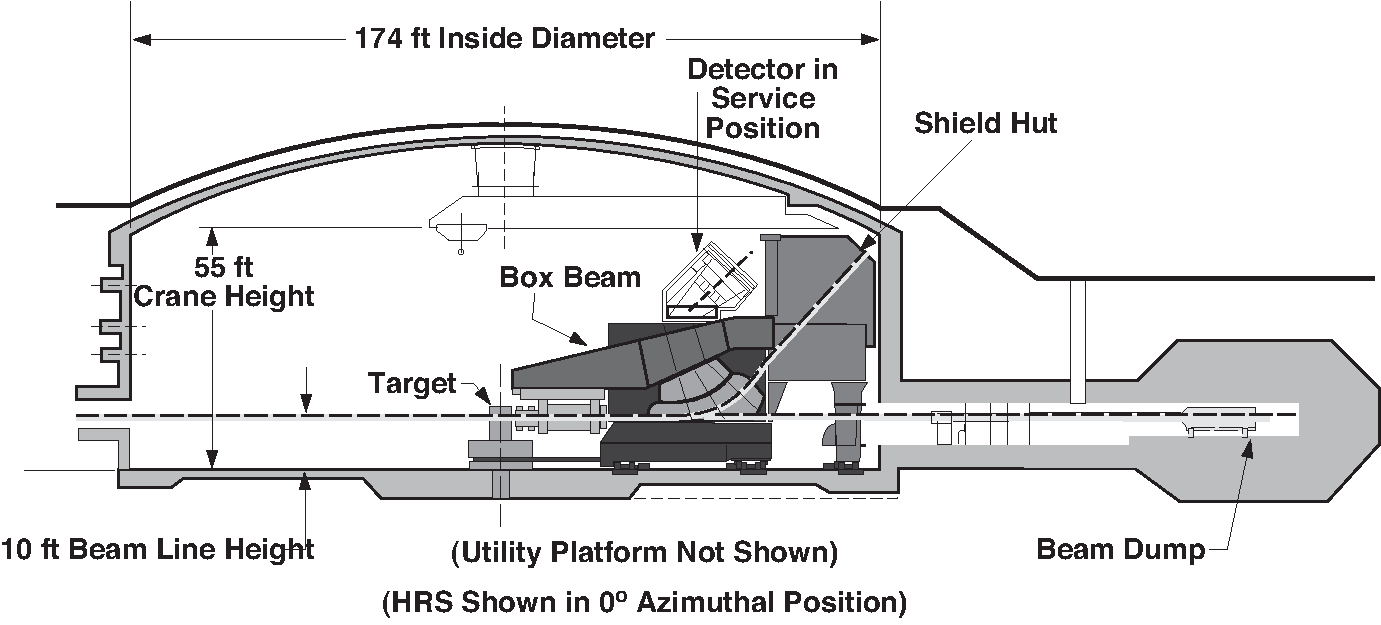
\includegraphics[width=0.75\textwidth]{./figures/halla_jlab/HallA}
  \caption[Side view of Hall-A]{Side view of Hall-A, which is a cylinder with 53 m in diameter and 17 m deep in the ground. The main instruments are the beamline components, the target system, two spectrometers and the beam dump. Figure is from Ref.~\cite{halla_nim}.}
  \label{sideview}
 \end{center}
\end{figure}
 Hall-A is a circular bulk (Fig.~\ref{sideview}) with a diameter of 53 m and a height of 17 m. The entire hall is buried underground and covered with concrete and earth. As shown in Fig.~\ref{topview}, the central elements in the hall include beamline components, a target system, and two identical high resolution spectrometers (HRSs). A detector package is stationed within a concrete shielding, called the detector hut, at the top of each HRS. The detector hut is designed to reduce the background in the detectors and protect them from radiation damage. Besides, it also stores electronic modules which collect signal outputs from detectors and the beamline, generate triggers, and provide the front end of the CEBAF Online Data Acquisition system (CODA). A detailed discussion of the Hall-A instrumentation is presented in the reference~\cite{halla_nim}.

\begin{figure}[!ht]
 \begin{center}
  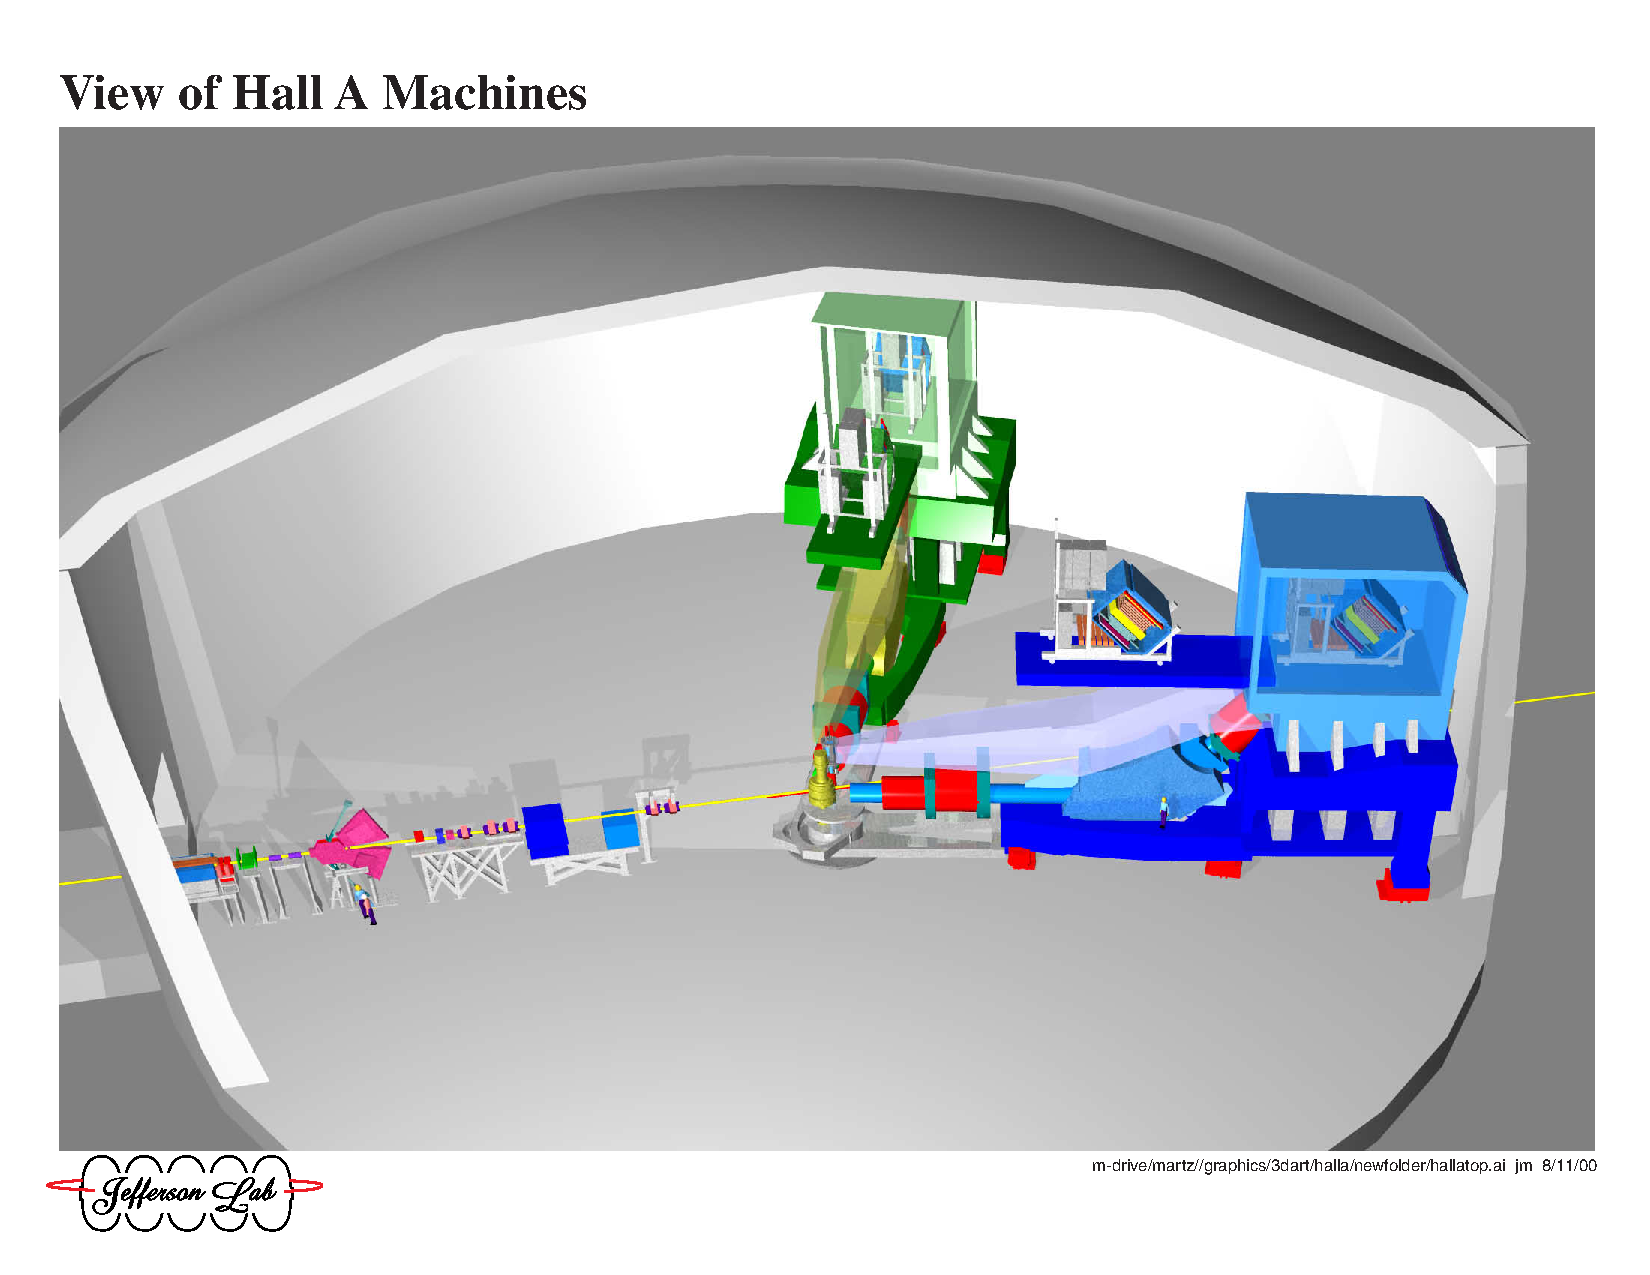
\includegraphics[width=0.75\textwidth]{./figures/halla_jlab/hallatop}
  \caption[Top view of Hall-A]{Top view of Hall-A. Two high resolution spectrometers are on each side of the beam line and can be rotated around the central pivot where the target chamber is installed. The detectors are located on top of each spectrometer and shielded by the detector hut.  Figure is from Ref.~\cite{halla_main}.}
  \label{topview}
 \end{center}
\end{figure}
%%%%%%%%%%%%%%%%%%%%%%%%%%%%%%%%%%%%%%%%%%%%%%%%%%%%
% Beam
%%%%%%%%%%%%%%%%%%%%%%%%%%%%%%%%%%%%%%%%%%%%%%%%%%%%
\section{Beam}
 The electron beam is delivered into Hall-A through a stainless steel tube which is 10 ft above the hall floor and holds a pressure $\mathrm{\leq 10^{-6}}$ Torr. The beam optics elements, including quadrupoles, sextupoles and corrector magnets, focus the beam on the target with spot sizes varying from 100 to 200 $\mathrm{\mu m}$ . A fast-raster system at 23 m upstream of the target position provides a beam spot of several millimeters at the target. As shown in Fig.~\ref{whole_beam}\cite{halla_nim}, the beam passing through the target is sent into the beam dump and spread out by a diffuser consisting of two 6.4~mm thick beryllium foils with water flowing between them. In addition, there are multiple beam diagnostics elements along the beamline to monitor, determine and control the relevant properties of the beam including the beam current, the beam position and direction, and the beam spot size at the target location. The energy and polarization of the electron beam are measured by individual methods and instruments~\cite{halla_nim}. 
\begin{figure}[!ht]
 \begin{center}
  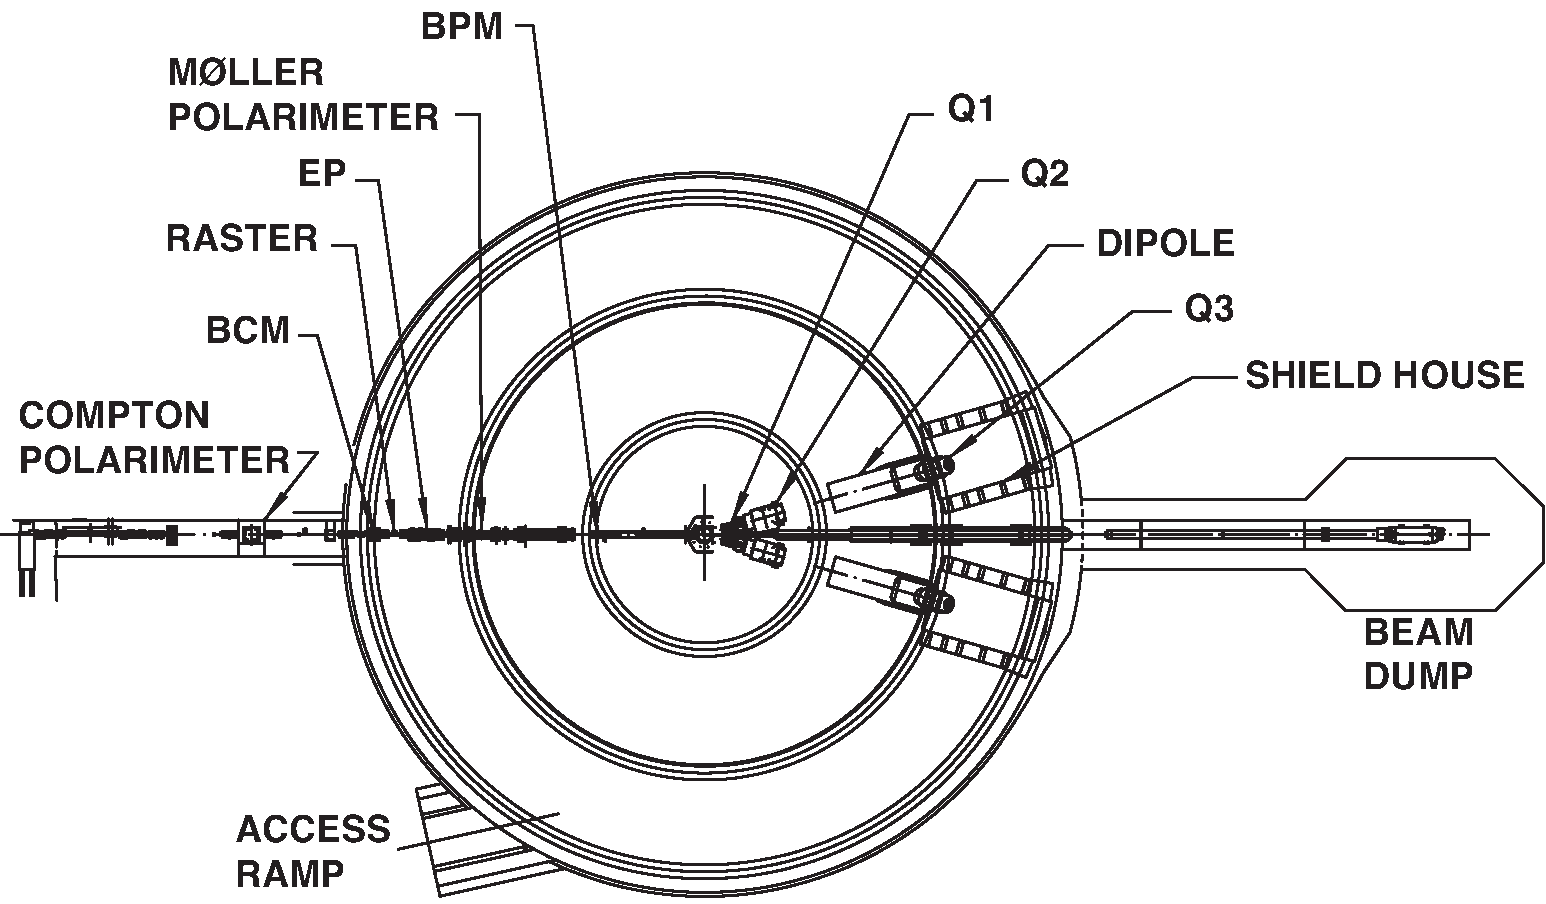
\includegraphics[width=0.6\textwidth]{./figures/halla_jlab/wholehall}
  \caption[Schematic layout of beam instruments and spectrometers in Hall-A]{\footnotesize{Schematic layout of beam instruments and spectrometers in Hall-A, including beamline components, beam diagnotistic elements,and beam dump. Figure is from Ref.~\cite{halla_nim}.}}
  \label{whole_beam}
 \end{center}
\end{figure}
\subsection{Beam Position Monitors}
 The position and direction of the beam at the target are determined by two beam position monitors (BPMs) located at 7.524~m and 1.286~m upstream of the target. Each BPM contains 4 antennas orientated orthogonally inside the beam pipe. Each antenna picks up a voltage reading from the beam when the beam current is above 1 $\mathrm{\mu A}$, and the signals from these antennas are used to calculate the beam position with the resolution of 100 $\mathrm{\mu m}$. The BPMs have to be calibrated independently to obtain the absolute position of the beam. When taking the calibration data, two pre-surveyed super-harps adjacent to BPMs are used to determine the absolute beam position~\cite{bpm_cali}. Event-by-event information from the BPMs is injected into the data stream, while the position average over every 0.3~s is also injected into the data stream every 3-4~s.

\subsection{Beam Charge Monitors}
The beam current monitor (BCM) is installed 25 m upstream of the target location and provides a non-interfering measurement of beam current. It consists of an Unser monitor, two RF cavities, several electronic modules and an associated DAQ system~\cite{halla_nim}. Two cavities on each side of the Unser monitor are high frequency wave-guides. The signal strength is proportional to the beam current when the cavities are tuned to the frequency of the beam. Before being sent into the RMS-to-DC converter~\cite{halla_nim}, each BCM output signal is split into three copies, two of which are amplified by 3 times and 10 times, respectively. Hence there are a total of six digital signals, $\mathrm{U_{1},~U_{3},~U_{10},~D_{1},~D_{3}}$ and $\mathrm{D_{10}}$, each of which is further divided into two copies and fed separately into scalers in HRSs. These digital signals are recorded by scalers in counts.

 During the data analysis, a BCM calibration is required to obtain the parameters to convert the scaler counts into electron charge. The procedure and result of the BCM calibration for this experiment can be found in Ref.~\cite{bcm_patricia}.
 
\subsection{Beam Energy}
The absolute energy of the beam can be determined by measuring the bend angle of the beam in the arc section of the beamline~\cite{beam_energy1,beam_energy2}. The momentum of the beam is related to the field integral of the eight dipoles and the bend angle:
\begin{equation}
  p = k \frac{\vec{B}\cdot \vec{dl}}{\theta},
\end{equation}
where $k\mathrm{=0.299792~GeV\cdot rad\cdot T^{-1}m^{-1}/c}$ and $\theta$ is the bend angle. The magnetic field integral of the eight dipoles are measured with respect to a reference dipole, the 9th dipole. The value of the bend angle is measured with a set of wire scanners.
 
%%%%%%%%%%%%%%%%%%%%%%%%%%%%%%%%%%%%%%%%%%%%%%%%%%%%
% Target
%%%%%%%%%%%%%%%%%%%%%%%%%%%%%%%%%%%%%%%%%%%%%%%%%%%%
\section{Target System}
 \begin{figure}[!ht]
 \begin{center}
  \includegraphics[angle=270,width=0.3\textwidth]{./figures/halla_jlab/cryotarget_loops}
  \caption[Picture of cryogenic target loops]{\footnotesize{Picture of cryogenic target loops, where Loop-1 and Loop-2 include 10 cm and 20 cm aluminium cells, respectively. Loop-3, which has two 20 cm cells, is not shown in this picture.}}
  \label{cryotarget_loop}
 \end{center}
\end{figure}
  The targets are located in a scattering vacuum chamber, which is supported by a 607~mm diameter central pivot connected to two HRSs. The main element within the scattering chamber is a cryogenic target system, which includes three loops of cryogenic targets, a target ladder to support solid targets, sub-systems for cooling and gas handling, temperature and pressure monitors, and target control and motion systems~\cite{halla_nim}. Three target loops are called Loop-1, Loop-2 and Loop-3. Both Loop-1 and Loop-2 contain two aluminium target cells with lengths of 10~cm and 20~cm, and Loop-3 has two 20~cm cells (Fig.~\ref{cryotarget_loop}).
\begin{figure}[!ht]
  \begin{center}
    \subfloat[First run period]{
      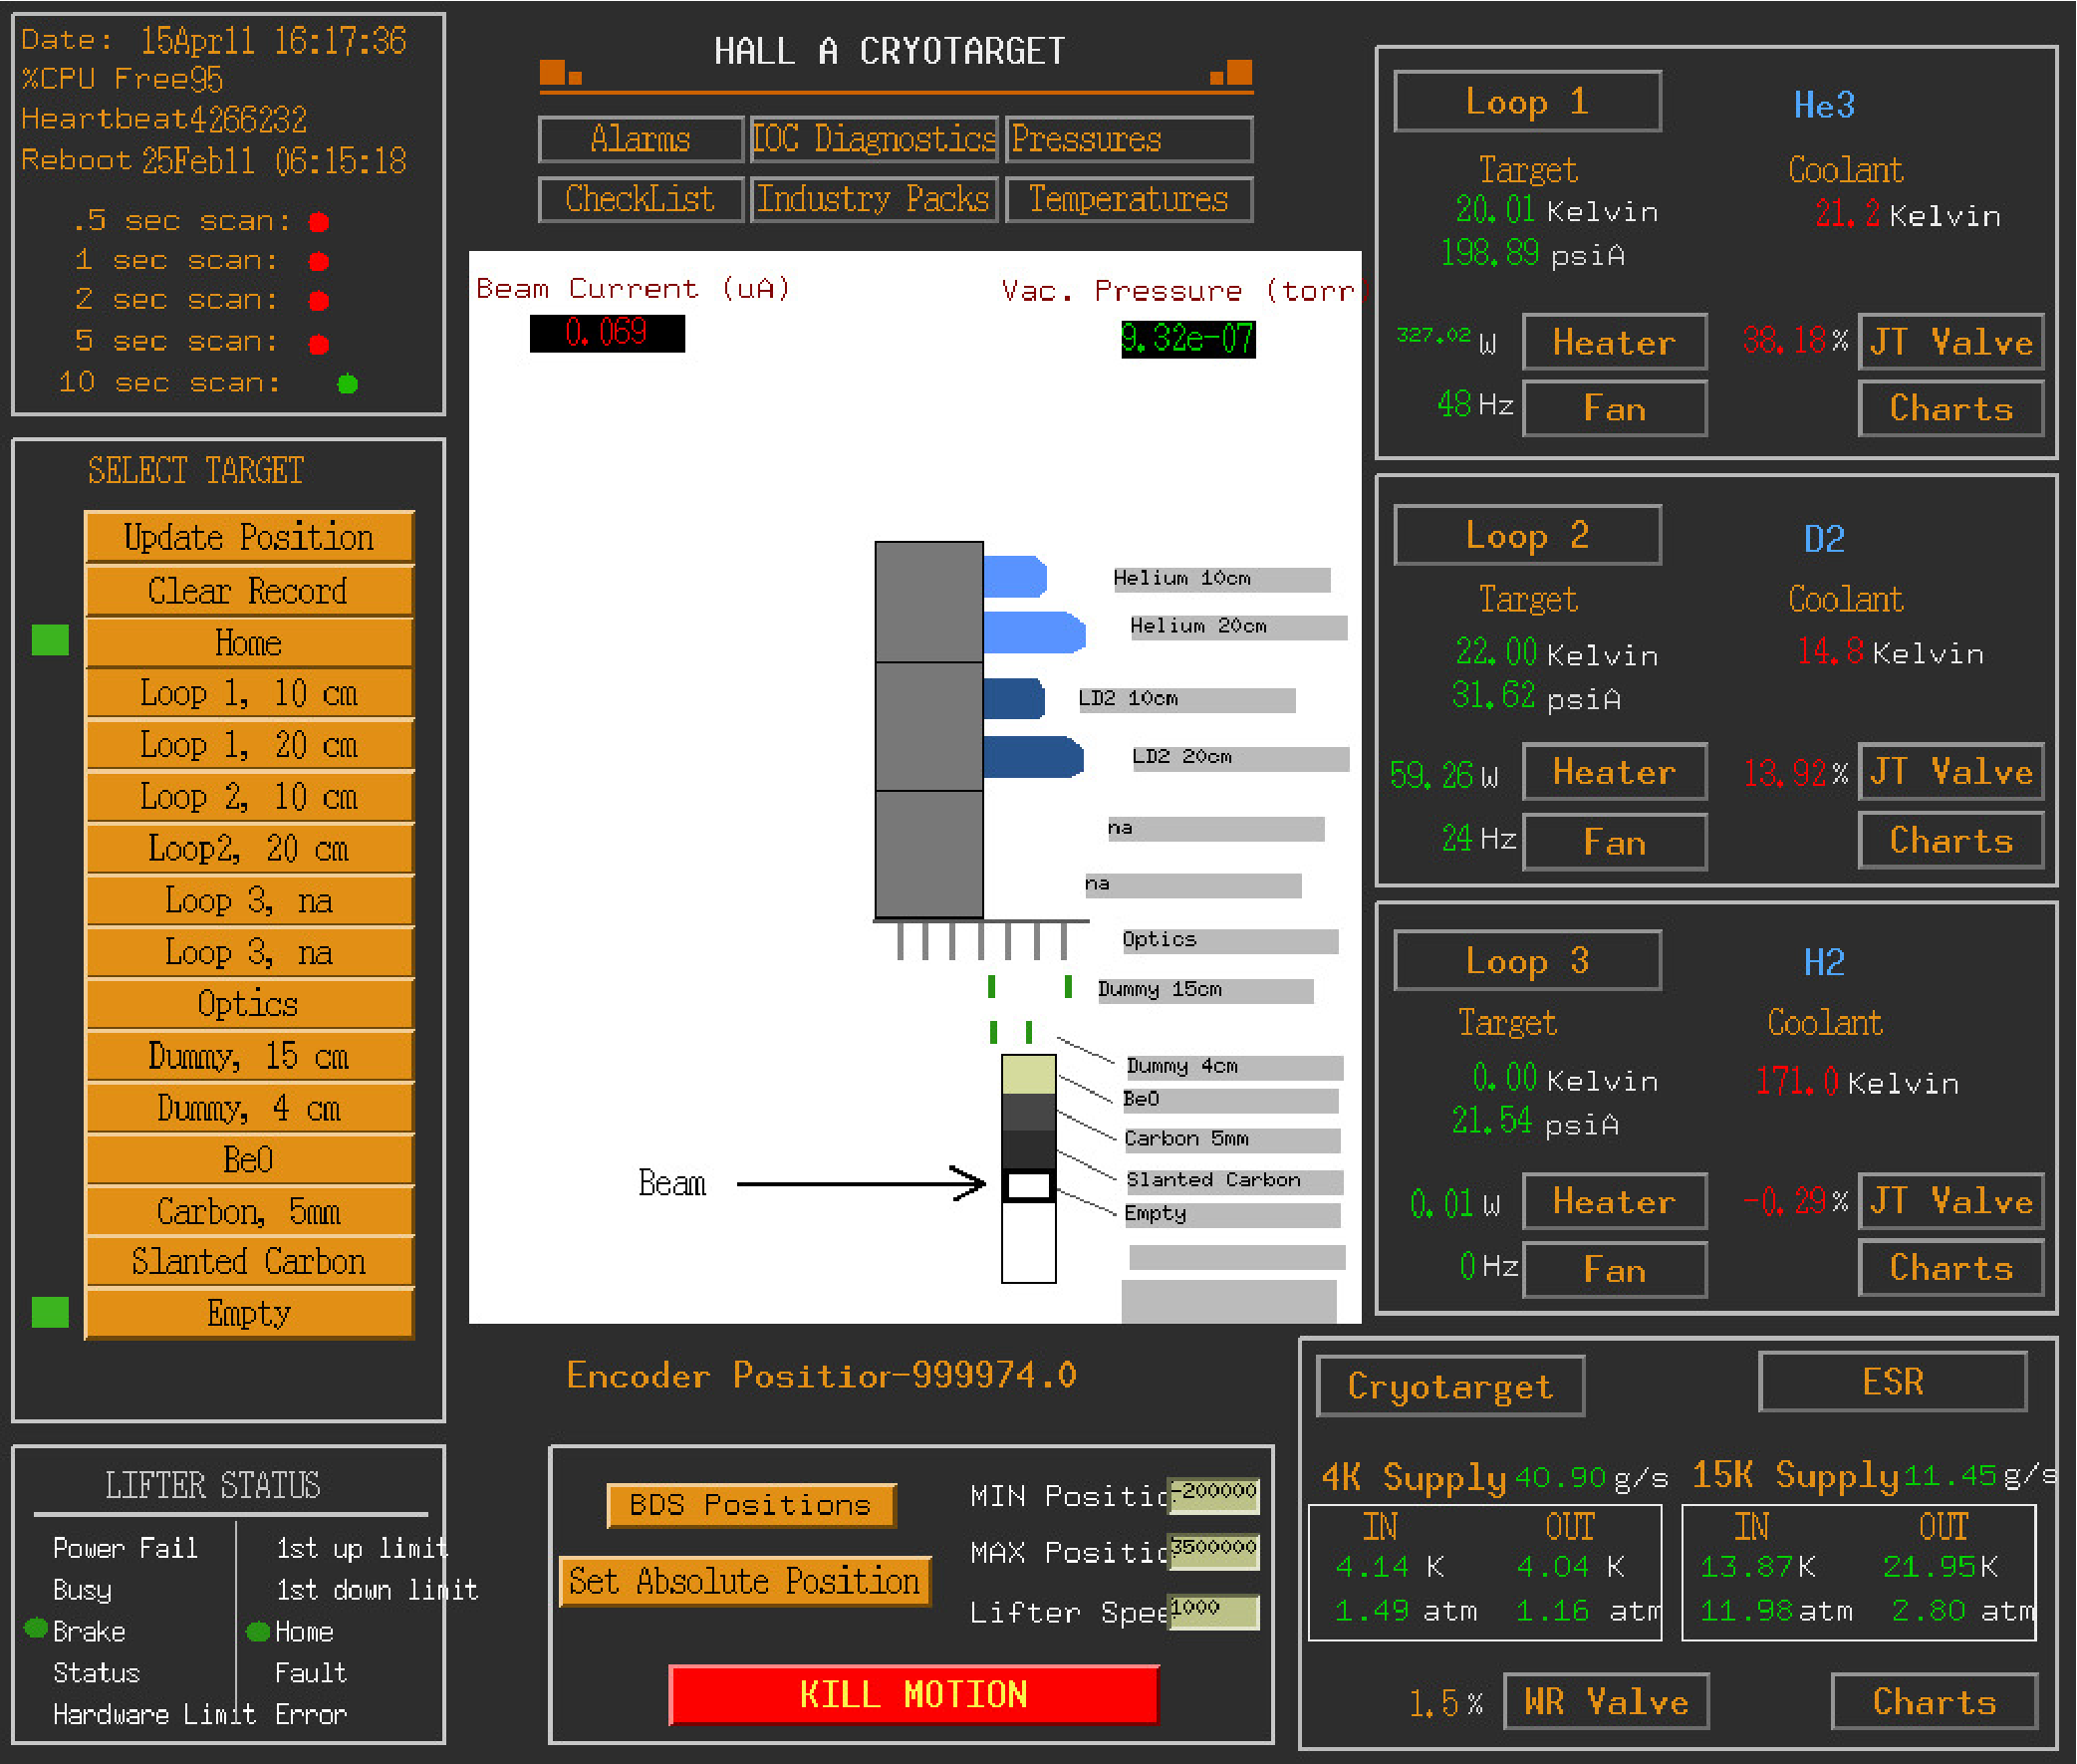
\includegraphics[type=pdf,ext=.pdf,read=.pdf,width=0.7\textwidth]{./figures/target/Target_First_Period}
      \label{target_run1}
    }
    \\
    \subfloat[Second run period]{
      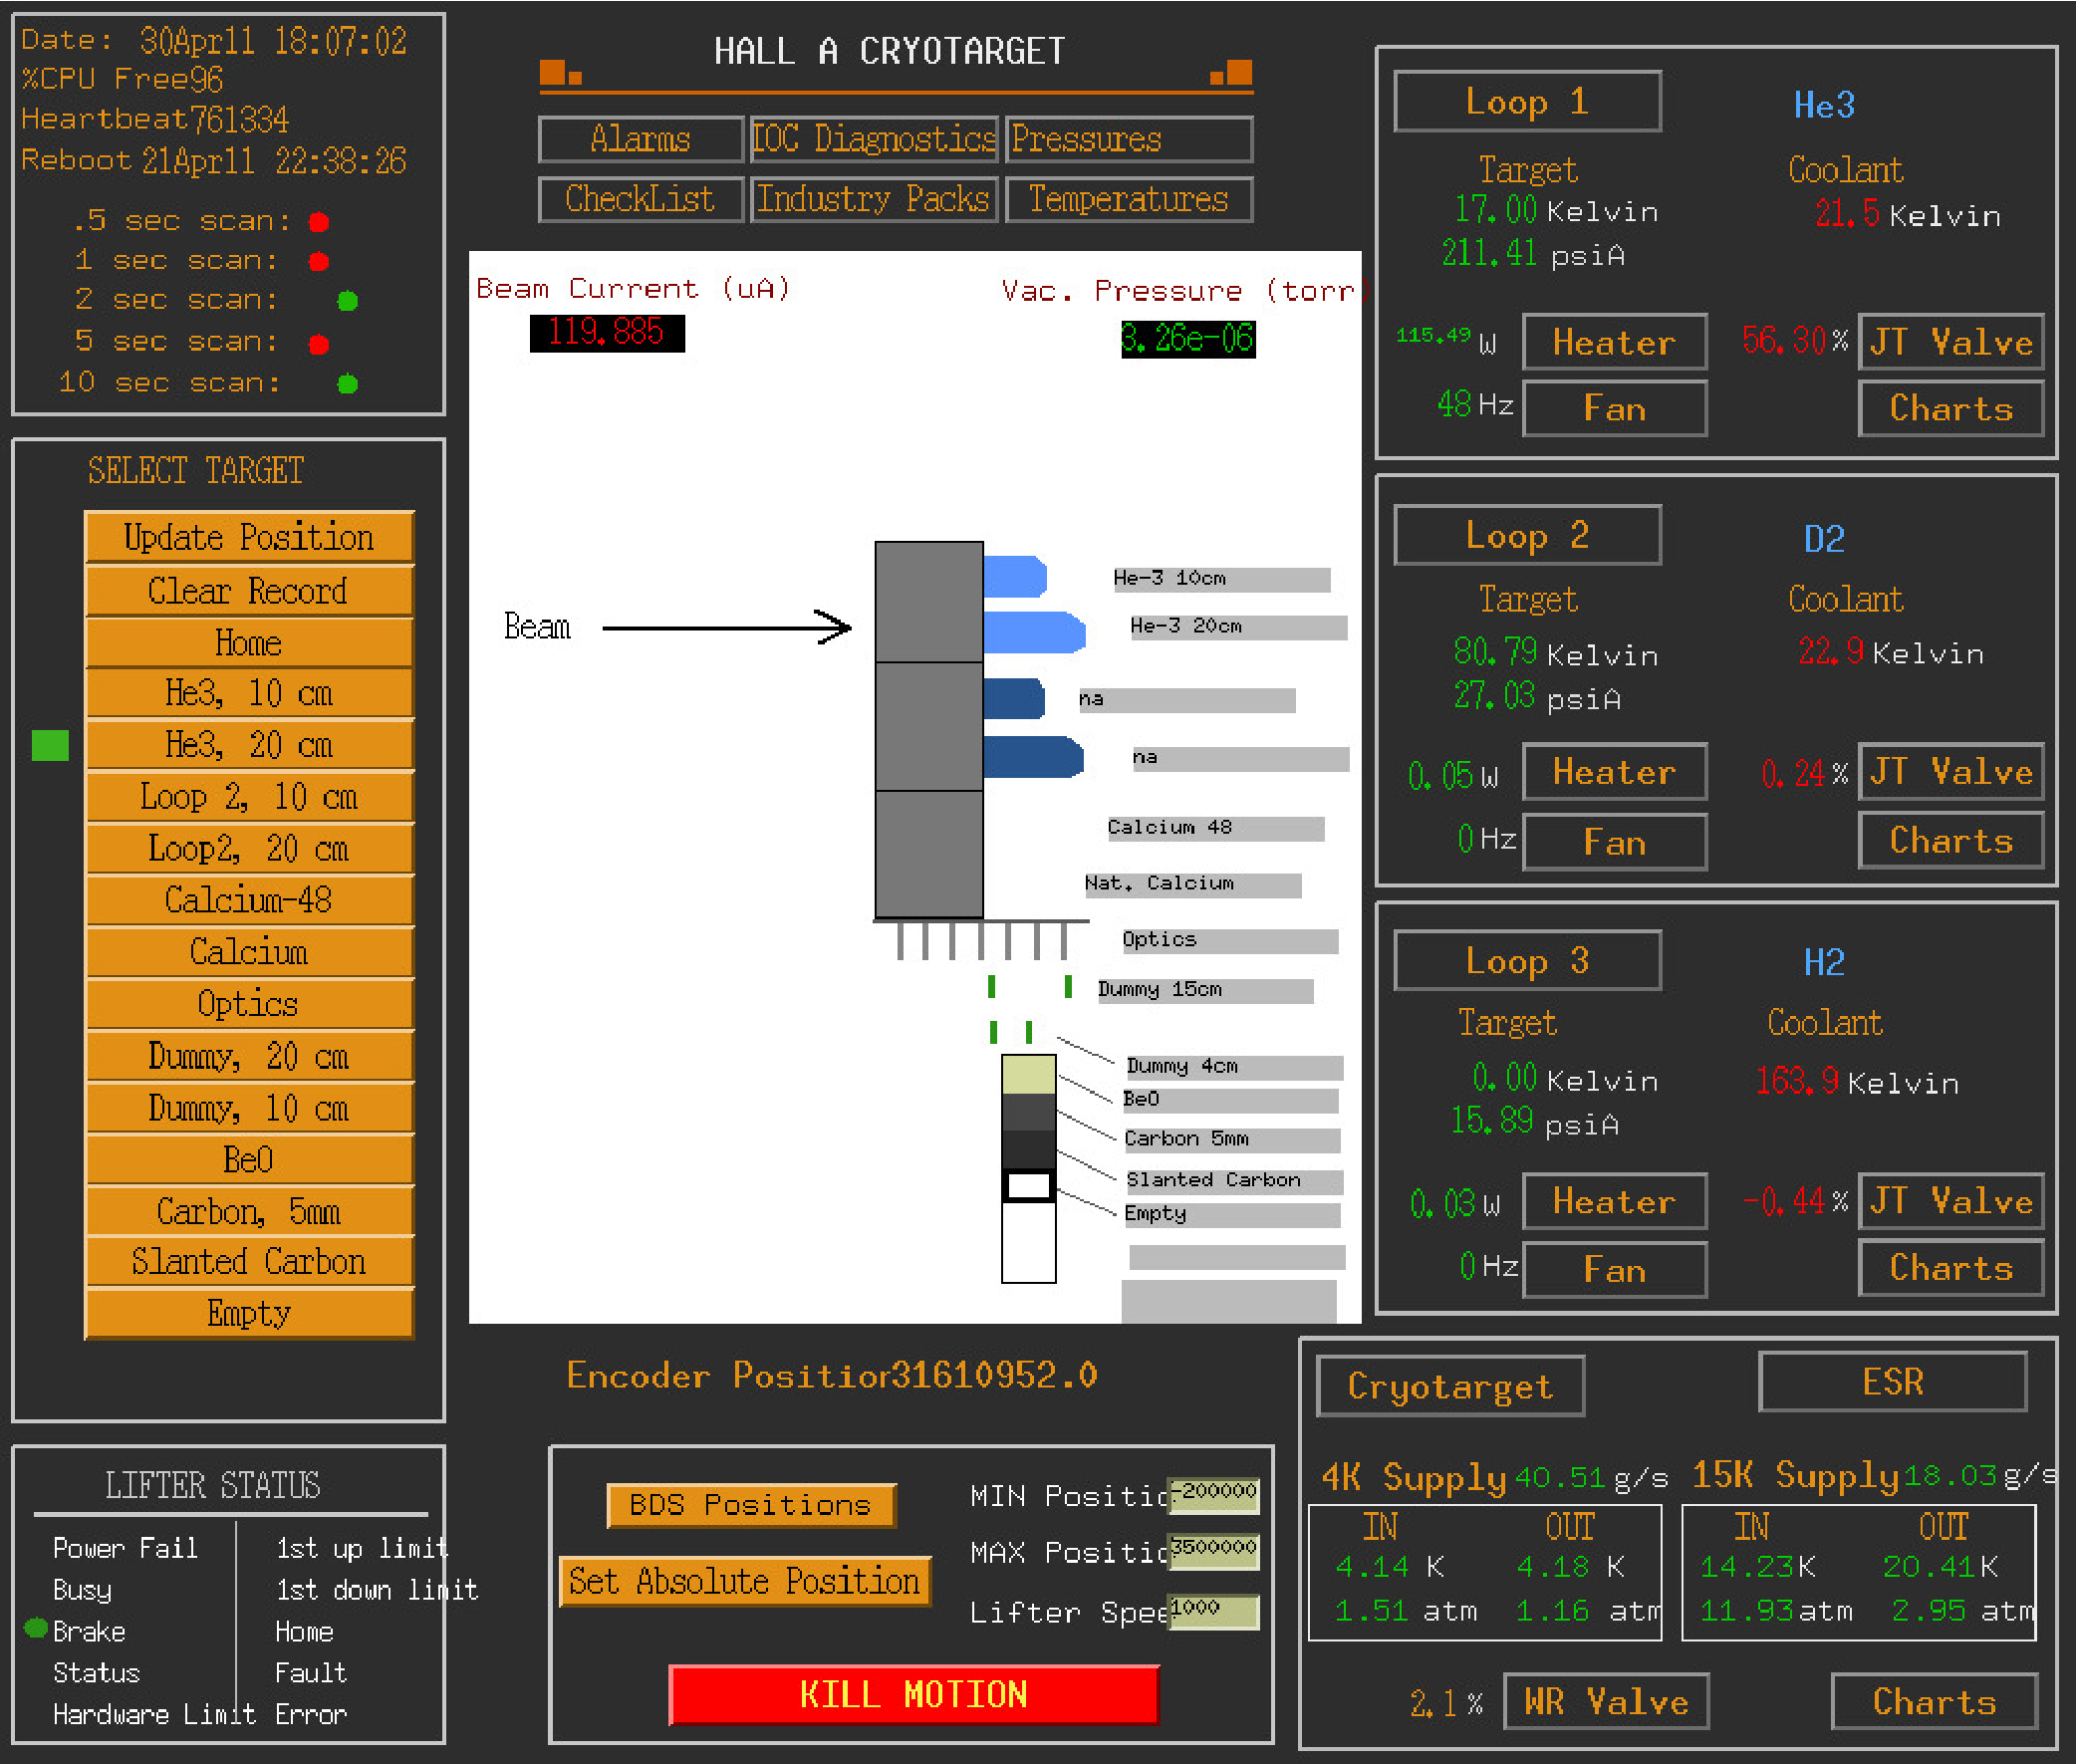
\includegraphics[type=pdf,ext=.pdf,read=.pdf,width=0.7\textwidth]{./figures/target/Target_Second_Period}
      \label{target_run2}
    }
    \caption[Target control screens]{\footnotesize{Target control screen. (a) shows the targets installed in the first run period and (b) shows the targets installed in the second run period. Figures were obtained during this experiment.}}
  \end{center}
\end{figure}

  The cryogenic targets used in this experiment were liquid deuterium ($\mathrm{LD_{2}}$), gaseous $\mathrm{^{3}He}$ and $\mathrm{^{4}He}$. In the first run period of this experiment (from April 15th 2011 to April 19th 2011), the 20~cm cells of Loop-1 and Loop-2 were filled with $\mathrm{^{4}He}$ and $\mathrm{LD_{2}}$, respectively. $\mathrm{^{4}He}$ was then replaced by $\mathrm{^{3}He}$ in the second run period (from April 21st 2011 to May 15th 2011), and $\mathrm{LD_{2}}$ was evacuated from Loop-2 (Fig.~\ref{target_run2}). Two 20 cm cells in Loop3 were used to store a $\mathrm{^{40}Ca}$ foil and a $\mathrm{^{48}Ca}$ foil which could not be directly exposed to the air. The temperature (pressure) of $\mathrm{LD{2}}$, $\mathrm{^{3}He}$ and $\mathrm{^{4}He}$ was maintained at 22~K (30.5 psia), 17~K (211 psia) and 20~K (202 psia), respectively. The cooling power was provided by the end station refrigerator (ESR)~\cite{cryo_grp} operated by the JLab cryogenic group. 
  \begin{table}[htbp]
   \begin{tabular}{lccccc}
   \toprule
   Target       &$\rho$ ($\mathrm{g/cm^{3}}$)& Length (cm)   & $\mathrm{\delta\rho}$ ($\mathrm{g/cm^{2}}$)& I ($\mathrm{\mu A}$)& Comment   \\
   \midrule
   $\mathrm{LD_{2}}$& 0.1676                 & 20.0          &     N/A                & 40          &Loop2      \\
   Al can (Loop-2)  & 2.7                    & 0.0272        &     0.0001             &             &  Entrance\\
                    & 2.7                    & 0.0361        &     0.0011             &             &  Exit     \\
                    & 2.7                    & 0.0328        &     0.0002             &             &  Wall     \\
   $\mathrm{^{3}He}$& 0.0296                 & 20.0          &     N/A                &120         &  Loop1    \\
   $\mathrm{^{4}He}$& 0.0324                 & 20.0          &     N/A                &90           &  Loop1    \\
   Al-can (Loop-1)  & 2.7                    & 0.0272        &     0.0002             &             &  Entrance \\
                    & 2.7                    & 0.0361        &     0.0006             &             &  Exit     \\
                    & 2.7                    & 0.0328        &     0.0005             &             &  Wall     \\
   $\mathrm{^{12}C}$&      2.265             & 0.3937        &     0.0008             &120          &           \\
   $\mathrm{^{40}C}$&      1.55              & 0.5735        &     0.01               &40           &  Loop3    \\
   $\mathrm{^{48}C}$&      1.55              & 0.5284        &     0.01               &40           &  Loop3    \\
   Al-can (Loop-3)  & 2.7                    & 0.0272        &     0.0001             &             &  Entrance \\
                    & 2.7                    & 0.0361        &     0.001             &              &  Exit     \\
                    & 2.7                    & 0.0328        &     0.0002             &             &  Wall     \\
   Dummy-20cm       &      2.7               & 0.1581        &     0.0005             &40           & Upstream  \\
                    &      2.7               & 0.1589        &     0.0005             &             & Downstream\\
   Dummy-10cm       &      2.7               & 0.1019        &     0.0003             &40           & Upstream  \\
                    &      2.7               & 0.1000        &     0.0003             &             & Downstream\\        
   \bottomrule
   \end{tabular}
  % \centering
  \caption[Targets in the E08-014]{\footnotesize{Targets in the E08-014, where BeO target and optics target are not listed. The detailed report is in Ref.~\cite{target_report}. The uncertainties of three cryo-targets are needed to be conformed so they are listed temporarily as "N/A". }}
  \label{target_table}
  \end{table}
  
   A 30~cm long optics target was installed right below Loop-3 for taking optics calibration data. The optics target contains 7 carbon foils located at -15 cm, -10 cm, -5 cm, 0 cm, 5 cm, 10 cm, and 15 cm, respectively. Two dummy targets, Dummy-20cm and Dummy-10cm, were installed below the optics target to measure contributions from the endcaps of the cryogenic target cells. Each of them contains two thick aluminium foils separated by 10~cm for Dummy-10cm and 20~cm for Dummy-20cm. There were three other targets, BeO, $\mathrm{^{12}C}$ and an empty target, installed on the target ladder below Dummy-10cm. 
 
  The list of targets used in this experiment is given in Table~\ref{target_table}. Detailed information of targets and related systems can be found in Ref.~\cite{target_report}. The target positions are typically surveyed during the preparation of the experiment. However, survey reports were only available for experiments that ran before this experiment, and the targets installed in the second run period were not surveyed. Their positions were extracted by comparing their positions, e.g. the positions of endcaps for cryo-targets, and the central foil of the optics target.
  
%%%%%%%%%%%%%%%%%%%%%%%%%%%%%%%%%%%%%%%%%%%%%%%%%%%%
% HRS
%%%%%%%%%%%%%%%%%%%%%%%%%%%%%%%%%%%%%%%%%%%%%%%%%%%%
\section{High Resolution Spectrometers}
\begin{figure}[!ht]
 \begin{center}
  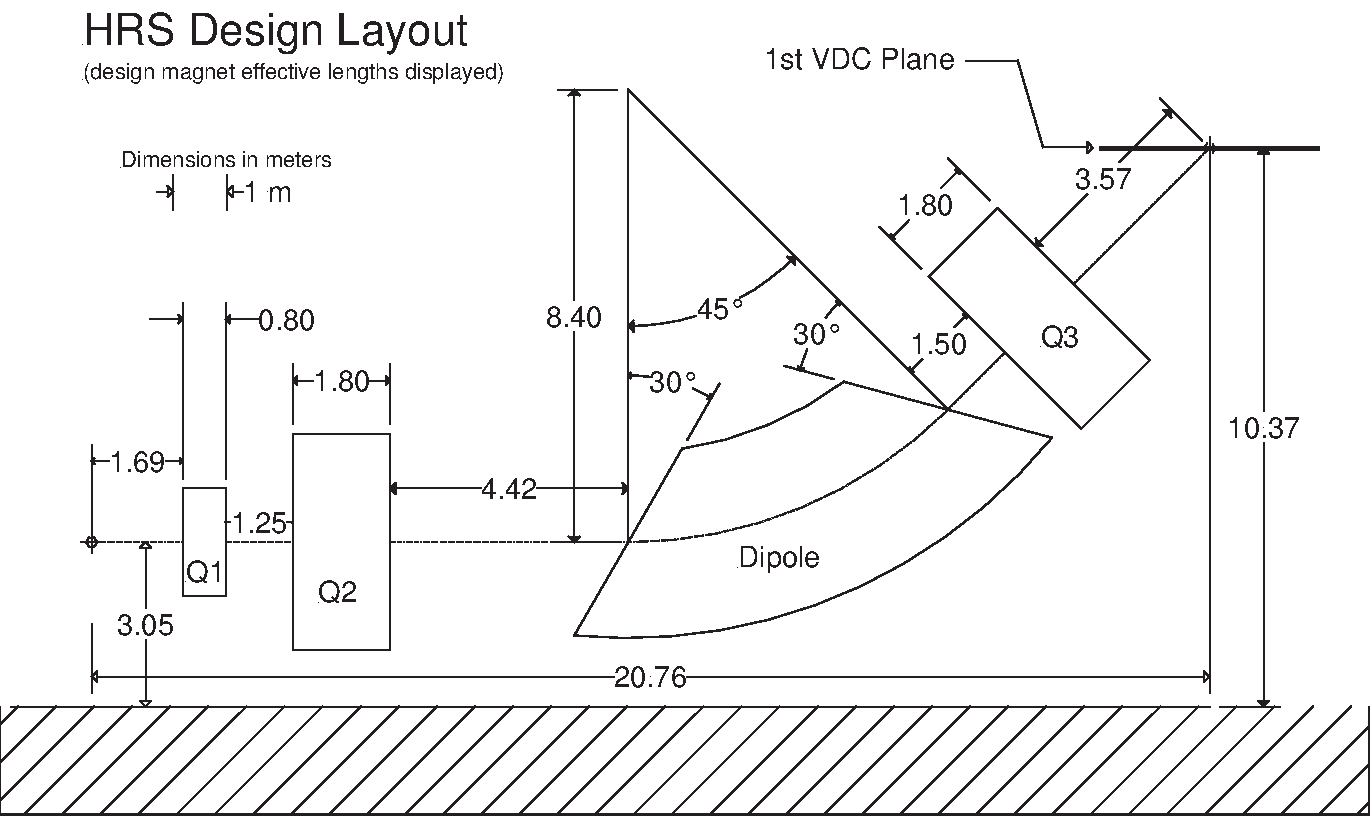
\includegraphics[width=0.8\textwidth]{./figures/halla_jlab/spectro}
  \caption[Schematic layout of HRS]{\footnotesize{Schematic layout of HRS, which shows the sizes and locations of the dipole and the three quadrupoles. Figure is from Ref.~\cite{halla_nim}.}}
  \label{halla_spectro}
 \end{center}
 \end{figure}
The essential equipments in Hall-A are two identical HRSs which provide high momentum resolution at the $\mathrm{10^{-4}}$ level over the range from 0.8 to 4.0~GeV/c, high position and angular resolution in the scattering plane, and large angular acceptance. As shown in Fig.~\ref{whole_beam}, the spectrometer on the left of the beam direction (to the beam dump) is called HRS-L, and the one on the right is called HRS-R. The basic layout of a HRS is given in Fig.~\ref{halla_spectro}. The magnet configuration of each HRS is QQDQ, including a dipole and three superconducting quadrupoles~\cite{halla_nim}. Two quadrupoles, Q1 and Q2, are installed in front of the dipole to achieve the desired angular acceptance and maximize the resolving power for the bend angle. The dipole performs a $\mathrm{45^{\circ}}$ vertical bending of the charged particles, and additionally, accommodates the extended targets and focuses the parallel beam. The third quadrupole, Q3, is behind the dipole to enhance the position and angular resolutions. Some important characteristics of the HRSs are listed in Table~\ref{hrs_table}.
 \begin{table}[htbp]
   \begin{tabular}{lcc}
   \toprule
   Bend Angle:           &$45^{\circ}$    \\   
   Optical Length:       &23.4 m      \\
   Momentum Range:       &0.3-4.0 GeV/c \\
   Momentum Acceptance:  &$-4.5\%<\delta p/p<+4.5\%$ \\
   Momentum Resolution:  &$1\times 10^{-4}$ \\
   Angular Range         &$12.5-150^{\circ}$ (HRS-L),12.5-130$^{\circ}$ (HRS-R) \\
   Angular Acceptance:   &$\pm$ 30~mrad (Horizontal), $\pm$ 60~mrad (Vertical)\\
   Angular Resolution:   &0.5 mrad (Horizontal), 1.0 mrad (Vertical)\\
   Solid Angle:          & 6 msr at $\delta p/p=0,y_{0}=0$\\
   Transverse Length Acceptance: &$\pm$ 5~cm \\
   Transverse Position Resolution: & 1 mm\\
   \bottomrule
   \end{tabular}
  % \centering
  \caption[Design characteristics of HRSs]{\footnotesize{Design characteristics of HRSs, where the resolution values are for the FWHM~\cite{halla_nim}.}}
  \label{hrs_table}
  \end{table}

 The power supply for the Q3 on HRS-R (RQ3) was not working properly during the experiment and limited the maximum central momentum setting to 2.876 GeV/c, but the experiment was planned to reach the maximum central momentum to 3.055~GeV/c. The RQ3 magnetic field was scaled down to 87.72\% at each kinematic setting. Accordingly, a new optics matrix was needed to match this new magnetic setting. An optics calibration to obtain the new matrix will be discussed in the next chapter.

%%%%%%%%%%%%%%%%%%%%%%%%%%%%%%%%%%%%%%%%%%%%%%%%%%%%
% Detector
%%%%%%%%%%%%%%%%%%%%%%%%%%%%%%%%%%%%%%%%%%%%%%%%%%%%
%\section{Detector Packages}
\input ./setup/setup_detector.tex

%%%%%%%%%%%%%%%%%%%%%%%%%%%%%%%%%%%%%%%%%%%%%%%%%%%%
% DAQ
%%%%%%%%%%%%%%%%%%%%%%%%%%%%%%%%%%%%%%%%%%%%%%%%%%%%
%\section{Data Acquisition System}
\input ./setup/setup_daq.tex
